\chapter{Radiaci\'{o}n de Hawking an\'{a}loga en sistemas ac\'{u}sticos}\label{cap2}
Como se observ\'{o} en el cap\'{i}tulo \ref{cap1}, la radiaci\'{o}n de Hawking tiene varios problemas para ser observada a nivel astrof\'{i}sico cuando los agujeros negros son creados por colapso gravitacional. Afortunadamente, \cite{Unruh1981} demostró que los agujeros negros no son los únicos objetos con la capacidad de emitir este tipo de radiaci\'{o}n. De hecho, en algunas condiciones (que se detallar\'{a}n más adelante) la física de las ondas que se propagan en fluidos cl\'{a}sicos o cu\'{a}nticos con movimiento tienen una correspondencia matemática con los campos cu\'{a}nticos que se propagan sobre una m\'{e}trica que describe un espacio-tiempo curvo por lo cual, pueden ser utilizados para realizar experimentalmente análogos del horizonte de un agujero negro en los que se podría observar el proceso de Hawking. Además, estos sistemas an\'{a}logos permiten hacer un corte en las frecuencias entrantes al horizonte debido que las ondas en un medio no existen para longitudes de onda cercanas o por debajo de cierta escala física. Por ejemplo, el sonido no se propaga por debajo de la distancia intermolecular típica de un fluido i.e., hay una frecuencia m\'{i}nima en nuestro modelo.

\section{Ondas sonoras en fluidos no Relativistas}
Partiremos explicando las ideas expuestas en  \citep{Unruh1981}, el cual es el art\'{i}culo  que da inicio a una nueva \'{a}rea de la f\'{i}sica moderna llamada \textit{gravedad an\'{a}loga} \citep{barcelo2011analogue} y en part\'{i}cular al tema de \textit{radiaci\'{o}n de Hawking  an\'{a}loga}.\\

Tomemos como sistema de trabajo un fluido no relativista, perfecto y barotr\'{o}pico. Con estas suposiciones, la din\'{a}mica de este sistema f\'{i}sico est\'{a} totalmente regida por las ecuaciones
\begin{align}\label{ec:fluid}
\partial_t \rho +\nabla .(\rho \textbf{v})=0,
\end{align}
\begin{align}\label{ec:fluido2}
\hspace{2.3cm} \partial_t\textbf{v}+(\textbf{v}.\nabla)\textbf{v}=-\frac{1}{\rho}\nabla p-\nabla \Phi,
\end{align}

donde $\textbf{v}(t,\textbf{r})$ es la velocidad del fluido, $\rho(t,\textbf{r})$ es su densidad, $p(t,\textbf{r})$ es la presi\'{o}n al cual est\'{a} sometido y $\Phi(\textbf{r})$ es un potencial externo. La ec. (\ref{ec:fluid}) expresa la conservaci\'{o}n de la masa, mientras que la ec. (\ref{ec:fluido2}) es la de Euler y representa la acci\'{o}n de fuerzas sobre el fluido. Adem\'{a}s, como el fluido es barotr\'{o}pico se tiene como funci\'{o}n de estado $p=p(\rho)$. Si adem\'{a}s $\textbf{v}$ es irrotacional, podemos definir un campo de velocidades $\psi$ tal que $\textbf{v}=\nabla \psi$.

\subsection{Linealizaci\'{o}n de las ecuaciones de campo}

Ahora supongamos que conocemos una solución $\psi_0,\rho_0, p_0$ que satisfacen las ecuaciones (\ref{ec:fluid}) y (\ref{ec:fluido2}). Nuestro inter\'{e}s es observar c\'{o}mo se modifica dicha soluci\'{o}n bajo una fluctuaci\'{o}n lineal, para ello proponemos una soluci\'{o}n general de la forma \citep{bookLandau}:

\begin{equation}
\begin{pmatrix}
\psi(\textbf{r},t)\\ 
\rho(\textbf{r},t)\\ 
p(\textbf{r},t)\\ 

\end{pmatrix}=\begin{pmatrix}
\psi_0(\textbf{r},t)\\ 
\rho_0(\textbf{r},t)\\ 
p_0(\textbf{r},t)\\ 

\end{pmatrix}+\begin{pmatrix}
\psi_1(\textbf{r},t)\\ 
\rho_1(\textbf{r},t)\\ 
p_1(\textbf{r},t)\\ 

\end{pmatrix}\epsilon+\vartheta(\epsilon^2),
\end{equation}
donde $\epsilon$ es un parámetro adimensional pequeño que no depende del tiempo y las coordenadas. Al linealizar la ecuaci\'{o}n de continuidad y expresar de forma lineal la dependencia de la presi\'{o}n y la densidad se tiene
\begin{align}
\nonumber  \partial_t \rho_1 +\nabla .(\rho_1 \nabla \psi_0+\rho_0\nabla \psi_1)&=0,\\
      p_1&=c^2\rho_1,
\end{align}\label{ec:fluidolin1}

con $ c^2=\frac{dp}{d \rho}(\rho_0)$ el cuadrado de la velocidad local de las perturbaciones lineales alrededor del campo de fondo $(\psi_0,\rho_0,p_0)$, i.e., es la velocidad del sonido propag\'{a}ndose en el fluido que esta en movimiento. La linealizaci\'{o}n de la ecuaci\'{o}n de Euler, requiere usar algunas identidades vectoriales como $(\textbf{v}.\nabla)\textbf{v}=\nabla \textbf{v}^2/2$ ya que $\nabla \times \textbf{v}=0$, adem\'{a}s $\nabla p_0=\nabla p(\rho_0)=c^2\nabla \rho_0$, y por tanto
\begin{equation}
\nabla(\partial_t \psi_1+ \nabla \psi_0.\nabla \psi_1)=-\nabla \Bigl(\frac{p_1}{p_0}\Bigr),
\end{equation}
que, despu\'{e}s de integrarse sobre todo el espacio equivale a
\begin{equation}\label{ec:eulerlineal}
\rho_0(\partial_t \psi_1+ \nabla \psi_0.\nabla \psi_1)=- p_1.
\end{equation}

Las ecuaciones diferenciales en \ref{ec:fluidolin1} y \ref{ec:eulerlineal} pueden combinarse y reescribirse como una \'{u}nica ecuaci\'{o}n diferencial de segundo orden que contiene la misma informaci\'{o}n
\begin{equation}\label{ec:campoescalar}
\partial_t\Bigl[\frac{\rho_0}{c^2}(\partial_t \psi_1+\nabla \psi_0 . \nabla \psi_1)\Bigr]=\nabla. \Bigl[\rho_0\nabla \psi_1-\frac{\rho_0}{c^2}\nabla \psi_0 (\partial_t \psi_1+\nabla \psi_0 . \nabla \psi_1)\Bigr].
\end{equation}
Esta es una ecuaci\'{o}n diferencial para el campo $\psi_1$ que se propaga sobre un fondo en movimiento, esta informaci\'{o}n est\'{a} contenida en los coeficientes de la ecuaci\'{o}n diferencial. Cuando el fondo es est\'{a}tico (no  fluye) $\nabla \psi_0=0$, la densidad volum\'{e}trica $\rho_0$ es estacionaria y homog\'{e}nea, i.e., la velocidad del sonido es la misma a todo tiempo y en todo el espacio. Con esto se encuentra que las perturbaciones acústicas del sistema se propagan como la luz en el vac\'{i}o a velocidad $c$ de acuerdo con la ecuación de d'Alembert:
\begin{equation}
\Bigl(-\frac{1}{c^2}\partial_{tt}+\nabla^2\Bigr)\psi=0.
\end{equation}
La ec. (\ref{ec:campoescalar}) se puede reescribir formalmente como
\begin{equation}
\frac{1}{\sqrt{-g}}\partial_{\mu}(\sqrt{-g}g^{\mu \nu}\partial_{\nu}\psi_1)=0,
\end{equation}
la cual describe la propagaci\'{o}n de un campo escalar libre y sin masa sobre un espacio-tiempo curvo. El espacio-tiempo aqu\'{i} representa el fluido en movimiento en el cual se propaga la perturbaci\'{o}n y la m\'{e}trica $g_{\mu \nu}$ es

\begin{align}
ds^2=g_{\mu \nu}dx^{\mu}dx^{\nu}=\frac{\rho_0}{c}\Bigl((c^2-\textbf{v}_0^2)dt^2+2\textbf{v}_0 \ddots \textbf{x}dt-d\textbf{x}\cdot \textbf{x}\Bigr).
\end{align}
Si se asume un medio esf\'{e}ricamente sim\'{e}trico estacionario y convergente, podemos definir un nuevo tiempo \citep{Unruh1981}:
\begin{equation}
\tau=t+\int \frac{v_0dr}{c^2-v_0^2},
\end{equation}
con lo cual la m\'{e}trica se reescribe como:
\begin{equation}\label{ec:metricafinal}
ds^2=\frac{\rho_0}{c}\Bigl((c^2-v_0^2)d\tau^2-\frac{cdr^2}{c^2-v_0^2}-r^2d\Omega^2\Bigr).
\end{equation}
Para que se emita radiaci\'{o}n de Hawking debe existir un horizonte y esto se consigue cuando la velocidad del flujo cambia suavemente tal que es igual a la velocidad del sonido $v_0=-c$ en alg\'{u}n punto $r=R$, por tanto
\begin{equation}
v_0=-c+\alpha(r-R)+\vartheta ((r-R)^2).
\end{equation}
Entonces la métrica anterior es \textit{an\'{a}loga} a la métrica de Schwarzschild (ver ec. (\ref{eqn:metricsc})) cerca al horizonte salvo una constante global, si el sistema no es homogen\'{e}no, aun as\'{i} las m\'{e}tricas son conformalmente equivalentes.\\

Por otro lado si $\psi_1$ es un campo cu\'{a}ntico que se propaga sobre un medio descrito por la m\'{e}trica ec. (\ref{ec:metricafinal}), tendremos los ingredientes b\'{a}sicos para predecir que los \textit{fonones} que se propagan fuera del horizonte poseen un espectro t\'{e}rmico caracterizado por una temperatura
\begin{equation}
T=\frac{\hbar}{2\pi\kappa_B}\alpha=\frac{\hbar}{2\pi\kappa_B}\left|\partial_r(v_0-c)\right|_{r=R},
\end{equation}
similar al caso de radiaci\'{o}n de Hawking descrito en el cap\'{i}tulo anterior donde al cambiar $\alpha\longrightarrow \kappa$ tenemos la misma expresi\'{o}n dada en la ec.(\ref{TH}).\\

El papel del horizonte de eventos en los agujeros negros an\'{a}logos lo desempeña ahora un horizonte acústico efectivo en el que la magnitud del flujo del medio es igual a la velocidad con la que se propaga una onda en el mismo medio. La visión crucial de Unruh en su trabajo del 1981 fue que una vez que se identifica que la propagaci\'{o}n de una onda sonora en un fluido es equivalente a la propagaci\'{o}n de la onda en un espacio-tiempo curvo, no queda m\'{a}s que repetir el argumento semiclásico de Hawking de 1975 para encontrar radiaci\'{o}n emitida cerca del horizonte, siendo la radiaci\'{o}n en el caso ac\'{u}stico fonones u ondas de sonido.


\section{An\'{a}logos de radiaci\'{o}n de Hawking en condensados de Bose-Einstein}

Gracias a los impresionantes avances en el enfriamiento y manipulación de gases atómicos ultrafríos, los experimentos son ahora capaces de  acceder a regímenes donde la materia es coherente, i.e., se logra tener un macroestado cu\'{a}ntico del sistema. En particular,  los BECs son una herramienta versátil para observar fluctuaciones cuánticas sobre este macroestado que describe el sistema. A saber, la radiación de Hawking de los agujeros negros acústicos es una de las más estudiadas te\'{o}ricamente y tal vez haya sido observada experimentalmente por \cite{de2019observation}.\\

En esta secci\'{o}n partiremos de la ecuaci\'{o}n fundamental que domina la din\'{a}mica de un fluido cu\'{a}ntico y encontraremos que una perturbaci\'{o}n sobre el fluido se comporta similar a un campo escalar propag\'{a}ndose en una m\'{e}trica efectiva. Adem\'{a}s, encontraremos la relaci\'{o}n de dispersi\'{o}n que siguen estas fluctuaciones, por \'{u}ltimo, aplicaremos estas ideas a la configuraci\'{o}n particular de l\'{a}ser de agujeros negros que permite autoamplificar la radiaci\'{o}n de Hawking.\\

Iniciemos recordando que un campo cu\'{a}ntico bos\'{o}nico  $\Psi$ cumple
\begin{eqnarray}\label{conmutador}
[\Psi(x,t),\Psi^{\dagger}(x',t)]=\delta(x-x'), \hspace{2cm} [\Psi(x,t),\Psi(x',t)]=0.
\end{eqnarray}
La primera es la relaci\'{o}n de conmutaci\'{o}n  can\'{o}nica y la segunda  es la conmutaci\'{o}n entre operadores de aniquilaci\'{o}n a tiempos iguales pero en puntos diferentes.\\
El campo cumple la ecuaci\'{o}n din\'{a}mica
\begin{equation}\label{ec:GP1}
i\hbar \partial_t \Psi=[\Psi,H],
\end{equation}
con el hamiltoniano
\begin{equation}
H=\int dx \Bigl[\frac{\hbar^2}{2m}\nabla_x\Psi^{\dagger} \nabla_x \Psi+ V\Psi^{\dagger}\Psi+\frac{g}{2}\Psi^{\dagger}\Psi^{\dagger}\Psi\Psi\Bigr].
\end{equation}
Primero verifiquemos que $\Psi$ cumple la ecuaci\'{o}n de Gross-Pitaevkii (GP), para lo cual observe que:
\begin{align*}
\nabla_x\cdot(\Psi^{\dagger}\nabla_x \Psi)=\nabla_x \Psi^{\dagger}\cdot\nabla_x\Psi+\Psi^{\dagger}\nabla_x^2\Psi,
\end{align*}
entonces
\begin{align*}
\nabla_x \Psi^{\dagger}\cdot \nabla_x\Psi=\nabla_x\cdot(\Psi^{\dagger}\nabla_x \Psi)-\Psi^{\dagger}\nabla_x^2\Psi,
\end{align*}
e integrando sobre un volumen ambos lados y usado el teorema de la divergencia
\begin{align*}
\int dx^3\ \nabla_x \Psi^{\dagger}\cdot\nabla_x\Psi=\int dS\ (\Psi^{\dagger}\nabla_x \Psi)-\int dx^3 \ \Psi^{\dagger}\nabla_x^2\Psi.
\end{align*}
La primera integral del lado derecho se anula en la superficie ya que los campos deben ser cero sobre la frontera, la amplitud del operador de campo es una funci\'{o}n de cuadrado integrable que expresa la probabilidad de aniquilar una part\'{i}cula en el punto $(x,t)$, el conjugado de esta funci\'{o}n expresa la probabilidad de crear una part\'{i}cula en el mismo punto. Con lo \'{u}ltimo se concluye que
\begin{equation}
\nabla_x \Psi^{\dagger}\cdot\nabla_x\Psi=-\Psi^{\dagger}\nabla_x^2\Psi,
\end{equation}
por tanto,
\begin{align}
\nonumber [\Psi,H]=&\int dx'\Bigl\{\Psi(x,t)\Psi(x',t)\Bigl[-\frac{\hbar^2}{2m}\nabla_x^2 + V+\frac{g}{2}\rho(x',t)\Bigr]\Psi(x',t)\\
\nonumber&-\Psi(x',t)\Bigl[-\frac{\hbar^2}{2m}\nabla_x^2 + V+\frac{g}{2}\rho(x',t)\Bigr]\Psi(x',t)\Psi(x,t)\Bigr\}\\
\nonumber=&\int dx'\Bigl\{ \Bigl(\delta(x-x')+\Psi(x',t)\Psi(x,t)\Bigr)\Big[...\Big]\Psi(x',t)-\Psi(x',t)\Psi(x,t)\Bigl[...\Bigr]\Psi(x',t)\Bigr\}\\
\nonumber =&\int dx'\Bigl\{ \delta(x-x')\Bigl[...\Bigr]\Psi(x',t)\Bigr\}\\
=&\Bigl[-\frac{\hbar^2}{2m}\nabla_x^2 + V+\frac{g}{2}\rho(x',t)\Bigr]\Psi(x,t),
\end{align}
remplazando el resultado anterior en la ec. (\ref{ec:GP1}) se obtiene la ecuaci\'{o}n de GP:
\begin{equation}\label{ec:GP2}
i\hbar\partial_t \Psi(x,t)=\Bigl(-\frac{\hbar^2}{2m}\nabla_x^2 + V+\frac{g}{2}\rho(x,t)\Bigr)\Psi(x,t),
\end{equation}
donde se ha definido $\rho\equiv|\Psi|^2$.\\

\subsection{Linealizaci\'{o}n de la ecuaci\'{o}n de campo}\label{Lcampo}
Si consideramos un campo que tiene peque\~{n}as fluctuaciones sobre el estado base, podemos escribir $\Psi$ como
\begin{equation}
\Psi=\psi(1+\Phi),
\end{equation}
donde $\psi$ es un campo cl\'{a}sico (funci\'{o}n escalar) y $\Phi$ representa la fluctuaci\'{o}n del campo (un campo cu\'{a}ntico).\\

¿Qu\'{e} ecuaci\'{o}n diferencial cumple el campo $\Phi$? Para responder esto iniciamos recordando las relaciones de conmutaci\'{o}n inicialmente expuestas se reescriben sobre la fluctuaci\'{o}n
\begin{align}
[\Phi(x,t),\Phi^{\dagger}(x',t)]=\delta(x-x') \qquad [\Phi(x,t),\Phi(x',t)]=0,
\end{align}
y el hamiltoniano

\begin{align}
\nonumber H=&\int dx \Bigl[\frac{\hbar^2}{2m}\nabla_x(\psi^*+\psi^*\Phi^{\dagger})\cdot\nabla_x(\psi+\psi\Phi)+V(\psi^*+\psi^*\Phi^{\dagger})(\psi+\psi\Phi)\\
\nonumber &+\frac{g}{2}(\psi^*+\psi^*\Phi^{\dagger})^2(\psi+\psi\Phi)^2\Bigr]\\
\nonumber =&\int dx \Bigl[\frac{\hbar^2}{2m}\Bigl(\nabla_x\psi^*\cdot\nabla_x \psi+\nabla_x\psi^*\cdot\nabla_x (\psi\Phi)+\nabla_x (\psi^*\Phi^{\dagger})\nabla_x\psi+\nabla_x(\psi\Phi^{\dagger})\cdot\nabla_x(\psi\Phi)\Bigr)\\
\nonumber &+V\rho_0\Bigl(1+ \Phi+\Phi^{\dagger}+\Phi^{\dagger}\Phi\Bigr)\\
 &+\frac{g}{2}\rho_0^2\Bigl(1+2\Phi+\Phi^2+2\Phi^{\dagger}+4\Phi^{\dagger}\Phi+2\Phi^{\dagger}\Phi^2+\Phi^{2\dagger}+2\Phi^{2\dagger}\Phi+\Phi^{2\dagger}\Phi^2\Bigr)\Bigr],
\end{align}
hemos definido $\rho_0\equiv|\psi|^2$ como la densidad de part\'{i}culas del campo cl\'{a}sico.  Reescribimos el hamiltoniano por partes, primero tomamos los t\'{e}rminos que no contienen $\Phi$,	 o de orden $0$
\begin{align}
H_0=&\int dx \Bigl[\frac{\hbar^2}{2m}\Bigl(\nabla_x\psi^*.\nabla_x \psi)+V\rho_0+\frac{g}{2}\rho_0^2\Bigr].
\end{align}
Luego tomamos los t\'{e}rminos que poseen orden lineal en $\Phi$:
\begin{align}
\nonumber H_1=&\int dx \Bigl\{\frac{\hbar^2}{2m} \Bigl(\nabla_x\psi^*.\nabla_x(\psi \Phi)+\nabla_x(\psi^* \Phi^{\dagger}).\nabla_x\psi+V\psi^*\psi(\Phi+\Phi^{\dagger})+\frac{g}{2}\rho_0\psi^*\psi(2\Phi+2\Phi^{\dagger})\Bigr\}\\
\nonumber =&\int dx\Big\{ \psi^*\Bigl[-\frac{\hbar^2}{2m} \nabla_x^2+V+g\rho_0\Bigr]\psi\Phi+\psi^*\Phi^{\dagger}\Bigl[-\frac{\hbar^2}{2m} \nabla_x^2+V+g\rho_0\Bigr]\psi\Bigr\}\\
=&\int dx\Big\{ \psi^*\Bigl[-\frac{\hbar^2}{2m} \nabla_x^2+V+g\rho_0\Bigr]+h.c.\Bigr\}.
\end{align}
Por \'{u}ltimo, tomamos los t\'{e}rminos de segundo orden (los de tercer y cuarto orden se desprecian)

\begin{align}
H_2=&\int dx \Bigl[\frac{\hbar^2}{2m} \nabla_x(\psi^*\Phi^{\dagger})\cdot\nabla_x(\psi\Phi)+V\rho_0\Phi^{\dagger}\Phi+\frac{g}{2}\rho_0^2(\Phi^2+\Phi^{2\dagger}+4\Phi^{\dagger}\Phi)\Bigr].
\end{align}
Analicemos el primer t\'{e}rmino:
\begin{align}
\nonumber \nabla_x(\psi^*\Phi^{\dagger})\cdot \nabla_x(\psi\Phi)=&(\nabla_x \psi^*\cdot\nabla_x\psi)\Phi^{\dagger}\Phi+\Phi^{\dagger}\nabla_x\psi^*\cdot\psi\nabla_x\Phi+\psi^*\nabla_x\Phi^{\dagger}\cdot(\nabla\psi)\Phi\\
\nonumber &+\psi^*\nabla_x\Phi^{\dagger}.\psi\nabla_x\Phi\\
\nonumber=&(\psi^*\nabla_x^2\psi)\Phi^{\dagger}\Phi+[\Phi^{\dagger}\nabla_x \psi^*\cdot\psi\nabla_x+\psi^*\nabla_x\Phi^{\dagger}\cdot\nabla_x\psi+\psi^*\nabla_x\Phi^{\dagger}\cdot\psi\nabla_x]\Phi\\
\nonumber=&(\psi^*\nabla_x^2\psi)\Phi^{\dagger}\Phi+[(\Phi^{\dagger}\nabla_x \psi^*+\psi^*\nabla_x\Phi^{\dagger})\cdot\psi\nabla_x+\psi^*\nabla_x\Phi^{\dagger}\cdot\nabla_x \psi]\Phi\\
\nonumber=&(\psi^*\nabla_x^2\psi)\Phi^{\dagger}\Phi+[\nabla_x(\Phi^{\dagger}\psi^*)\cdot\psi\nabla_x)+\psi^*\nabla_x\Phi^{\dagger}\cdot\nabla_x\psi]\Phi\\
\nonumber=&\Phi^{\dagger}(\psi^*\nabla_x^2\psi)\Phi+\nabla_x(\Phi^{\dagger}\psi^*)\cdot\psi\nabla_x\Phi+\psi^*\nabla_x\Phi^{\dagger}\cdot\nabla_x\psi\Phi\\
=&\Phi^{\dagger}(\frac{\psi}{\psi}\psi^*\nabla_x^2\psi)\Phi+\Phi^{\dagger}\nabla_x \psi^*\psi\nabla_x\Phi-\frac{2mv}{\hbar}i\nabla_x \Phi,
\end{align}
con lo anterior, el hamiltoniano se reescribe como
\begin{align}
\nonumber H_2=&\int dx \rho_0\Bigl\{\Phi^{\dagger}\Bigl[\frac{-\hbar^2}{2m\rho_0} \nabla_x(\rho_0\nabla_x)-iv\hbar\nabla_x-\frac{\hbar^2}{2m}\frac{\nabla^2\psi}{\psi}+V+2g\rho_0\Bigr]\Phi\\
\nonumber &+\frac{g}{2}\rho_0(\Phi^2+\Phi^{2\dagger})\Bigr\}.
\end{align}
Por tanto $H=H_0+H_1+H_2$, tal que la ecuaci\'{o}n din\'{a}mica para el campo ahora es
\begin{align}
\nonumber i\hbar\partial_t(\psi+\psi\Phi)=&[\psi+\psi\Phi,H_0+H_1+H_2]\\
=&[\psi,H_0]+[\psi,H_1]+[\psi,H_2]+[\psi\Phi,H_0]+[\psi\Phi,H_1]+[\psi\Phi,H_2],
\end{align}
los tres primeros conmutadores son nulos por que $\psi$ es una funci\'{o}n escalar, el cuarto se anula por que $H_0$ no depende de $\Phi$. Por tanto
\begin{equation}
i\hbar \partial_t \psi+i\hbar\partial_t(\psi)\Phi+i\hbar\psi\partial_t\Phi=\psi[\Phi,H_1]+\psi[\Phi,H_2],
\end{equation}

con lo que podemos dividir el problema en
\begin{equation}\label{a1}
i\hbar\partial_t\psi=\psi[\Phi,H_1]
\end{equation}
\begin{equation}\label{a2}
\hspace{1.9cm} i\hbar\partial_t\Phi=[\Phi,H_2]-i\hbar\partial_t\psi/\psi,
\end{equation}

resolviedo la ec. (\ref{a1}), se encuentra la ecuaci\'{o}n din\'{a}mica para el campo $\psi$ que es la ecuaci\'{o}n de GP que se encontr\'{o} al inicio y era de esperar dado que describe la din\'{a}mica del macroestado del sistema. Resolviendo la ec. (\ref{a2}) se tiene


\begin{align}
\nonumber [\Phi,H_2]=&\int dx'\rho_0\Bigl\{\Phi(x,t)\Phi^{\dagger}(x',t)\Bigl[...\Bigr]\Phi(x',t)+\frac{g}{2}\rho_0\Phi(x,t)(\Phi^2+\Phi^{2\dagger})\\
\nonumber &-\Phi^{\dagger}(x',t)\Bigl[...\Bigr]\Phi(x',t)\Phi(x,t)+\frac{g}{2}\rho_0(\Phi^2+\Phi^{2\dagger})\Phi(x,t)\Bigr\}\\
\nonumber =&\int dx'\rho_0\Bigl\{\Bigl(\delta(x-x')+\Phi^{\dagger}(x',t)\Phi(x,t)\Bigr)\Bigl[...\Bigr]\Phi(x',t)\\
\nonumber &+\frac{g}{2}\rho_0\Phi(x,t)(\Phi^2+\Phi^{2\dagger})\Bigr\}-\Phi^{\dagger}(x',t)\Bigl[...\Bigr]\Phi(x',t)\Phi(x,t)-\frac{g}{2}\rho_0(\Phi^2+\Phi^{2\dagger})\Phi(x,t)\Bigr\}\\
\nonumber =&\Bigl[...\Bigr]\Phi(x,t)+\int dx'\rho_0\Bigl[\Bigl\{\Phi^{\dagger}(x',t)\Phi(x,t)\Bigl[...\Bigr]\Phi(x',t)-\Phi^{\dagger}(x',t)\Phi(x,t)\Bigl[...\Bigr]\Phi(x',t)\Bigr\}\\
&+\frac{g}{2}\rho_0\Phi(x,t)(\Phi^2+\Phi^{2\dagger})-\frac{g}{2}\rho_0(\Phi^2+\Phi^{2\dagger})\Phi(x,t)\Bigr],
\end{align}
el t\'{e}rmino entre corchetes cuadrados dentro de la integral es el nulo. Aplicando con cuidado los propiedades de conmutaci\'{o}n, se obtiene
\begin{align}
[\Phi,H_2]=\Bigl[...\Bigr]\Phi(x,t)+\frac{2g}{2}\rho^2\Phi^{\dagger},
\end{align}
por tanto
\begin{align}\label{ec:bogoliubov}
\nonumber i\hbar\partial_t \Phi=&\left(\frac{-\hbar^2}{2m\rho_0}\nabla_x(\rho_0\nabla_x)-iv\hbar\nabla_x-\frac{\hbar^2}{2m}\frac{\nabla_x^2 \psi}{\psi}+V+2g\rho_0\right)\Phi\\
\nonumber &+g\rho_0\Phi^{\dagger}-\left(\frac{-\hbar^2}{2m}\frac{\nabla_x^2 \psi}{\psi}+V+g\rho
_0\right)\Phi\\
=& \left(\frac{-\hbar^2}{2m\rho_0}\nabla_x(\rho_0\nabla_x)-iv\hbar\nabla_x\right)\Phi+g\rho_0(\Phi^{\dagger}+\Phi).
\end{align}
Esta ecuaci\'{o}n gobierna la din\'{a}mica de una fluctuaci\'{o}n creada sobre el macroestados que describe el condensado.
\subsection{Relaci\'{o}n de dispersi\'{o}n}\label{fluctuacion}
Para encontrar c\'{o}mo se mueven la fluctuaciones $\Phi$, asumimos que el operador de campo puede descomponerse en modos de frecuencia $\omega$, tal que
\begin{equation}\label{ec:antza}
\phi_{\omega}(t,x)=a_{\omega}\exp[-i\omega t]\phi_{\omega}(x)+a^{\dagger}_{\omega}\Bigl[\exp[-i\omega t]\varphi_{\omega}(x)\Bigr]^{*},
\end{equation}
donde $a$ y $a^{\dagger}$ son los operadores de aniquilación y creación de fonones. Insertando  la ec. (\ref{ec:antza}) en la ec. (\ref{ec:bogoliubov}), se tiene

\begin{align}\label{ec:l2}
\nonumber \left[\hbar(\omega+iv\partial_x)+\frac{\hbar^2}{2m\rho_0}\partial_x\rho_0\partial_x-mc^2\right]\phi_{\omega}&=mc^2\varphi_{\omega},\\
\left[-\hbar(\omega+iv\partial_x)+\frac{\hbar^2}{2m\rho_0}\partial_x\rho_0\partial_x-mc^2\right]\varphi_{\omega}&=mc^2\phi_{\omega},
\end{align}
donde se ha definido $c^2=g\rho_0/m$ como la velocidad que lleva la fluctuaci\'{o}n sobre el fluido. Para obtener la relaci\'{o}n de dispersi\'{o}n, consideremos una región en la que el condensado es homogéneo ($\rho_0$ constante) y busquemos soluciones de las ec. (\ref{ec:l2}) en forma de ondas planas $\phi_{\omega}\propto \varphi_{\omega} \propto\exp[ikx]$. Destacamos que la frecuencia $\omega$ y
el número de onda $k$ no están restringido a valores reales por tanto pueden ser complejos, m\'{a}s adelante se ver\'{a} el motido de esta afirmaci\'{o}n. Las partes imaginarias de $\omega$ y $k$ codificarán el comportamiento dinámico del sistema y es lo que se estudiar\'{a} en el pr\'{o}ximo cap\'{i}tulo. Sustituyendo lo mencionado en las ecs. (\ref{ec:l2}) se obtiene

\begin{equation}
\begin{pmatrix}
\hbar(\omega-v k)-\displaystyle \frac{\hbar}{2m}k^2-mc^2 &-mc^2\\
-mc^2&-\hbar(\omega-vk)-\displaystyle \frac{\hbar}{2m}k^2-mc^2
\end{pmatrix}\begin{pmatrix}
\phi_{\omega}\\
\varphi_{\omega}
\end{pmatrix}=\begin{pmatrix}
0\\
0  
\end{pmatrix}.
\end{equation}
Los t\'{e}rminos fuera de la diagonal mezclan modos de frecuencia negativa y positiva, entre los que se incluyen el proceso de Hawking. Para que exista una solución no trivial, el determinante de la matriz anterior debe ser nulo, esto conduce inmediatamente a la relación de dispersión de Bogoliubov.
\begin{equation}\label{ec:disper}
(\omega-v k)^2=c^2 k^2+\frac{\hbar^2k^4}{4m^2}=F^2(k),
\end{equation}
se acostumbra escribir $k^2_0=4m^2/(\hbar^2c^2)=2/\xi^2$, donde $\xi$ se conoce como la longitud de restituci\'{o}n (\textit{healing length}) y define la escala de Planck efectiva en los an\'{a}logos de gravedad en BECs. Este tipo de dispersi\'{o}n se conoce como \textit{an\'{o}mala}\footnote{Una relaci\'{o}n de dispersi\'{o}n an\'{o}mala se refiere al crecimiento de la velocidad de grupo cuando crece la frecuencia.} y es globalmente válida en condensados homogéneos. En configuraciones no homogéneas sigue siendo válida como una relación de dispersión estrictamente local, siempre que todas las cantidades involucradas $(c, v$ y $k$) varíen lentamente con $x$. En la ec. (\ref{ec:disper}) $\omega$ representa la frecuencia de la fluctuaci\'{o}n en el marco de laboratorio y $F(k)$ es la frecuencia en el marco com\'{o}vil (marco que se mueve con la velocidad del fluido).\\

Observe que la relaci\'{o}n de dispersi\'{o}n anterior es cu\'{a}rtica en $k$  indicando que el modo $\phi$ para una frecuencia $\omega$ fija es:
\begin{equation}
\phi=\exp[-i\omega t]\sum_j A_j \exp[i k_j x].
\end{equation}
Por otro lado, la ec. (\ref{ec:disper}) que siguen peque\~{n}as fluctuaciones presentes en un BEC puede igualmente derivarse de la ecuaci\'{o}n de movimiento para una fluctuaci\'{o}n en un campo de velocidades (una onda de sonido) en un fluido irrotacional que incluye la dispersi\'{o}n de Bogoliubov
\begin{align}\label{ec:dinamica}
(\partial_t+\partial_x v)(\partial_t+v\partial_x)\phi=\partial_x^2\phi-\frac{1}{k_0^2}\partial_x^4\phi.
\end{align}
Alternativamente, la anterior ecuaci\'{o}n se puede obtener proponiendo una acci\'{o}n adecuada para el campo \citep{Corley1999}:
\begin{equation}
S_{\phi}=\frac{1}{2}\int d^2x\Bigl([(\partial_t+v\partial_x)\phi]^2+\phi\Bigl[\partial_x^2-\frac{1}{k_0^2}\partial_x^4\Bigr]\phi\Bigr).
\end{equation}
El operador $\partial_t+v\partial_x$ es la derivada temporal en el marco com\'{o}vil o del fluido, es decir, $d/dt=\partial_t+v\partial_x$. A partir de la acci\'{o}n podemos verificar que \'{e}sta es invariante bajo transformaciones de fase si el campo escalar es complejo. Esto implica una corriente conservada $j^{\mu}$, la cual alquiere importancia porque su componente temporal permite definir el producto interno 
\begin{equation}\label{ec:norma1}
(\phi_1,\phi_2)=-i\int dx[\phi_1^*(\partial_t+v\partial_x)\phi_2-\phi_2(\partial_t+v\partial_x)\phi_1^{*}],
\end{equation}
la cual es una cantidad conservada, i.e., $\partial_t(\phi_1,\phi_2)=0$ cuando $\phi_1$ y $\phi_2$ son soluciones a la ec. (\ref{ec:dinamica}). En consecuencia, la norma $(\phi_1,\phi_1)$ de una soluci\'{o}n $\phi_1$ de la ec. (\ref{ec:dinamica}) es igualmente conservada. La conservación del producto escalar y de la norma en particular permite la creaci\'{o}n de part\'{i}culas por la existencia de modos negativos durante el proceso de Hawking.\\

En este trabajo $v$ tomar\'{a} dos valores diferentes constantes tal que dividir\'{a} el espacio en dos regiones, una subs\'{o}nica $v_1<c$ y otra supers\'{o}nica $v_2>c$. Con esto de forma general un modo se puede escribir como $\exp[ikx-i\omega t]$ para modos contrapropagantes y $\exp[-ikx-i\omega t]$ para modos copropagantes. Con $\omega=\pm vk+F(k)$, donde $(+)$ corresponde a modos contrapropagantes y $(-)$ a modos copropagantes.\\

Si se normalizan los modos con respecto al producto escalar, la ecuaci\'{o}n ec. (\ref{ec:norma1}) se reescribe como

\begin{align}\label{ec:norma}
\Bigl(\exp[\pm ik_1x-i(vk_1+F(k_1))t],\exp[\pm ik_2 x-i(vk_2+F(k_2))t]\Bigr)=4\pi F(k)\delta(k_1-k_2)
\end{align}
La norma es positiva si $F$ es positivo, con lo cual, cuando $\omega$ es positiva se encontrar\'{a}n dos modos con norma positiva en la rama copropagante denotados por (v) en la relaci\'{o}n de dispersi\'{o}n y dos modos en la rama contrapropagantes denotados por (u). La norma es negativa si $F$ es negativa y aqu\'{i} si $\omega$ es positiva solo se encontr\'{a}n dos modos en la rama contrapropagante (u) (ver figura \ref{fig:2.1}). En el cap\'{i}tulo \ref{cap3} se aclar\'{a} con m\'{a}s detalle esta afirmaci\'{o}n.
\subsection{An\'{a}lisis por teor\'{i}a de inestabilidades}\label{sec:Inestabilidad}
Las inestabilidades en dinámica de fluidos se pueden introducir a partir de la siguiente pregunta: ¿qué sucede cuando peque\~{n}as fluctuaciones aparecen en un fluido que est\'{a} en movimiento?, ¿las perturbaciones crecen o decaen a trav\'{e}s del tiempo? En el caso de que las fluctuaciones crezcan decimos que el fluido es inestable, si las perturbaciones decaen, llamamos al fluido estable \citep{koschmieder1977instabilities}. ¿Qu\'{e} pasa en un fluido cu\'{a}ntico como los BECs? Suponiendo una pequeña fluctuaci\'{o}n $\Phi$ sobre el estado macrosc\'{o}pico del sistema $\psi$, se encuentra que la fluctuaci\'{o}n  se rige por la ecuaci\'{o}n lineal ec. (\ref{ec:bogoliubov}) y los valores propios ec. (\ref{ec:disper}) deciden su evoluci\'{o}n.\\

Las frecuencias propias complejas con partes imaginarias positivas son las que indican inestabilidades porque permiten que la fluctuci\'{o}n que se genera espont\'{a}neamente en el sistema crezca en el el tiempo. ¿C\'{o}mo ver que la  ec. (\ref{ec:bogoliubov}) acepta soluciones con frecuencias complejas? Para observar esto definamos las dos componentes del campo como
\begin{eqnarray}
W=\begin{pmatrix}
\Phi\\
\Phi^{\dagger}

\end{pmatrix}.
\end{eqnarray}
Para un estado estacionario la  ec. (\ref{ec:bogoliubov}) se puede reescribir como
\begin{align}\label{ec:Hermi}
i \hbar \partial_t W= \omega W=B W,
\end{align}
con el operador $B$ siendo representado por
\begin{equation}
B=\Bigl(\frac{-\hbar^2}{2m\rho_0}\nabla_x(\rho_0\nabla_x)+g\rho_0\Bigr)\sigma_3-iv\nabla_x+ig\rho_0\sigma_2,
\end{equation}
donde $\sigma_i$ son las matrices de Pauli
\begin{eqnarray}
\sigma_1=\begin{pmatrix}
0&1\\
1&0
\end{pmatrix}, \hspace{0.5cm}
\sigma_2=\begin{pmatrix}
0&-i\\
i&0
\end{pmatrix}, \hspace{0.5cm}
\sigma_3=\begin{pmatrix}
1&0\\
0&1
\end{pmatrix}.
\end{eqnarray}
La ec. (\ref{ec:Hermi}) indica que $\omega$ es una cantidad conservada y que el operador $B$ no es herm\'{i}tico por el t\'{er}mino $ig\rho_0\sigma_2$, i.e., sus valores propios pueden ser complejos, por tanto $\omega=\omega_R+i\omega_I$. La inestabilidad se encuentra cuando fijamos $\omega_I>0$ y ser\'{a} tema de discusi\'{o}n en el cap\'{i}tulo \ref{cap3}.

\section{Configuraci\'{o}n de l\'{a}ser de agujeros negros (BHL)}\label{BHL}

En presencia de dos horizontes, ciertas condiciones permiten amplificar la radiaci\'{o}n de Hawking (RH) de manera similar a un l\'{a}ser. Por esta raz\'{o}n este fen\'{o}meno es conocido como l\'{a}ser de agujeros negros (BHL) y es una manera de validar experimentalmente los resultados de Hawking y es una propuesta tratada de forma controversial por \cite{Steinhauer2014} por que sus resultados experimentales de la funci\'{o}n de correlaci\'{o}n han sido obtenidos con simulaciones puramente cl\'{a}sicos de BECs \textit{Manuele Tettamant, private communication 2019}, \citep{tettamanti2016numerical},\citep{steinhauer2017self}.\\

Esta idea de BHL es publicada por primera vez por \citep{Corley1999} qui\'{e}nes demuestran que en presencia de dos horizonte, uno interno u horizonte de agujero blanco (WH) y otro externo u horizonte de agujero negro (BH) la RH sufre un proceso de autoamplificaci\'{o}n si el campo a tratar es bos\'{o}nico y la relaci\'{o}n de dispersi\'{o}n es an\'{o}mala. En el caso que el campo sea de fermiones, la radiaci\'{o}n es atenuada.\\ Esta estimulaci\'{o}n (si el campo es bos\'{o}nico) o supresi\'{o}n (si el campo es fermi\'{o}nico) de la RH es una consecuencia del \textit{confinamiento} de las part\'{i}culas con frecuencia negativa en la regi\'{o}n entre los horizontes.\\

Para entender este fen\'{o}meno  se tomar\'{a} como campo bos\'{o}nico las fluctuaciones que se generan en un BEC, estudiadas en la secci\'{o}n \ref{fluctuacion}. El elemento de l\'{i}nea en la ec. (\ref{ec:metricafinal}) se reducir\'{a} a 1+1 dimensi\'{o}n obteniendo $ds^2=c^2dt^2-(dx-v(x)dt)^2$, el cual es suficiente para ilustrar la f\'{i}sica detr\'{a}s del BHL. El perfil de velocidades $v(x)$ se asume negativo (es decir el fluido se mueve a la izquierda), este fluido tiene una velocidad constante  $v_1<0$ excepto en el interior de los horizontes donde el valor ser\'{a} $v_2$ con $v_2<v_1$ entre $x_{WH}$ y $x_{BH}$ (con $x_{WH}<x_{BH}$).\\

En la figura \ref{fig:2.1}(b) el movimiento del fluido est\'{a} descrito por el perfil de velocidades $v(x)$ m\'{a}s simple posible para un BHL, este perfil suele ser llamado plano \citep{2012Larre}. Los horizontes definen tres regiones: la regi\'{o}n I o zona subs\'{o}nica donde la velocidad del fluido es menor a la velocidad de la perturbaci\'{o}n ($v_1<c)$. La regi\'{o}n II o zona supers\'{o}nica, definida como el interior de los horizontes y es donde la velocidad del fluido es mayor a la velocidad de las perturbaciones ($v_2>c$). Por \'{u}ltimo la regi\'{o}n III, donde el sistema tiene la misma configuraci\'{o}n que en la regi\'{o}n I, i.e., es subs\'{o}nica.\\


 \begin{figure}
 
   \centering
   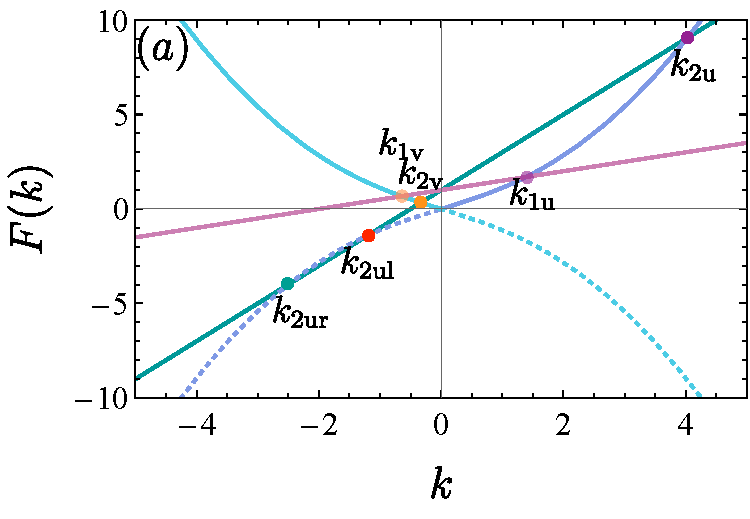
\includegraphics[height=5cm]{f21a.pdf}%
   \hspace{0.1cm}% add some horizontal spacing
   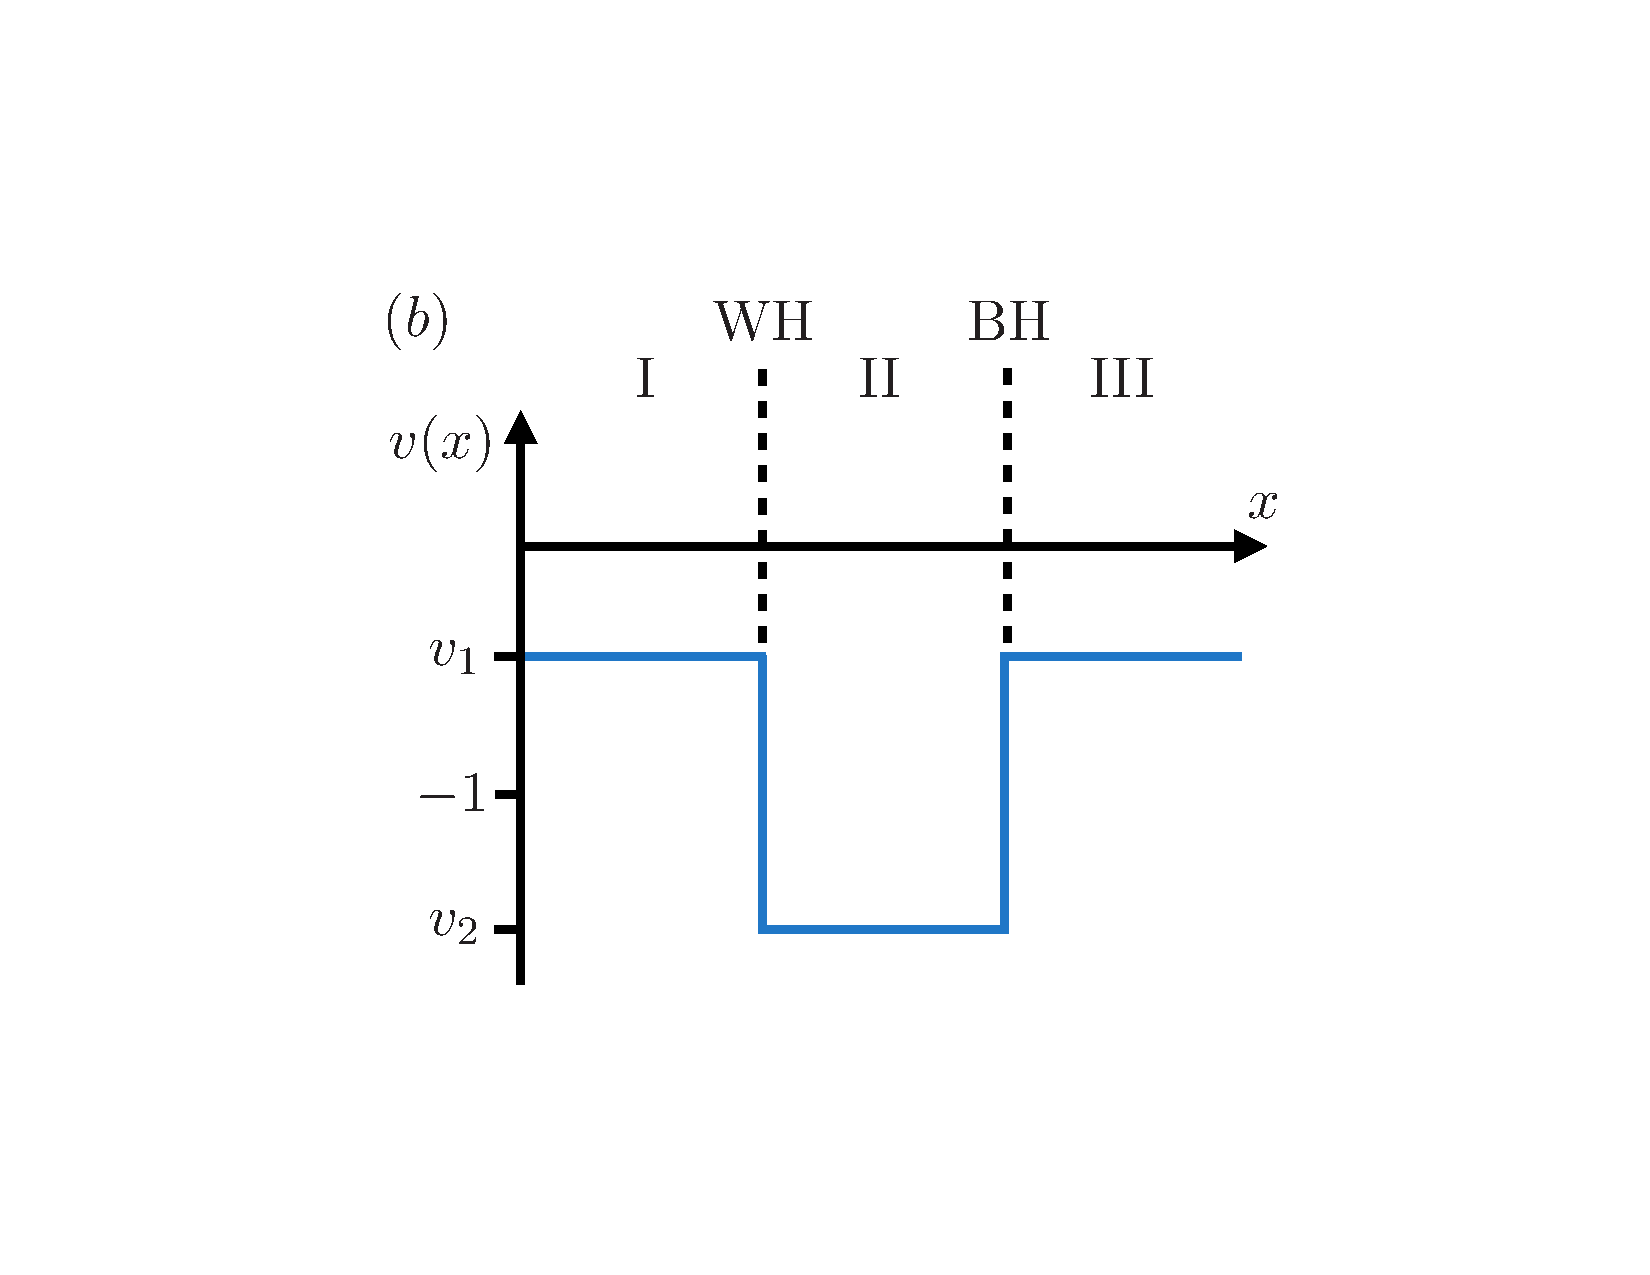
\includegraphics[height=5cm]{Fig21.pdf}%
   \caption{(a) Relaci\'{o}n de dispersi\'{o}n en el marco com\'{o}vil. En morado se encuentra la rama que contiene modos contrapropagantes, mientras de azul la rama con modo copropagantes. La solución gráfica para dos perfiles de velocidad: una subsónica $v_1$ (rosa) y otra supersónica $v_2$ (verde). Aquí $v_1= -1$, $k_0 = 2$, $c = 1$, $v_2= - 2$ y $\omega=1$. (b) Perfil de velocidades del fluido $v(x)$ para las tres regiones, I y III con velocidad subs\'{o}nica y II con velocidad supers\'{o}nica \citep{2018Bermudez}.} 
   \label{fig:2.1}
\end{figure}

\subsection{Propagaci\'{o}n de una onda plana a trav\'{e}s del BHL}

Ahora que se tiene en mente la configuraci\'{o}n del BHL,  es natural preguntarse qu\'{e} le pasa a una onda plana con frecuencia $\omega$ y n\'{u}mero de onda $k$ que es soluci\'{o}n a la relaci\'{o}n de dispersi\'{o}n  ec. (\ref{ec:disper}) cuando se encuentra dentro de la cavidad. Para dar una respuesta inicialmente cualitativa a esta pregunta, supongamos que iniciamos con el modo $k_{\text{2ul}}$, que es soluci\'{o}n a la relaci\'{o}n de dispersi\'{o}n y de la ec.(\ref{ec:norma}) $F(k)<0$ por tanto su norma es negativa, vea figura \ref{fig:2.1}(a). Esta soluci\'{o}n se encuentra en la rama contrapropagante (u) de la relaci\'{o}n de dispersi\'{o}n, adem\'{a}s como est\'{a} dentro de la cavidad, es decir en la regi\'{o}n II o supers\'{o}nica es nombrado con el sub\'{i}ndice ($2$u), la velocidad de grupo de este modo es $d\omega/dk<1$ por tanto se mueve a la izquierda por lo que la \'{u}ltima etiqueta de este modo es $l$.\\
\begin{figure}\centering
	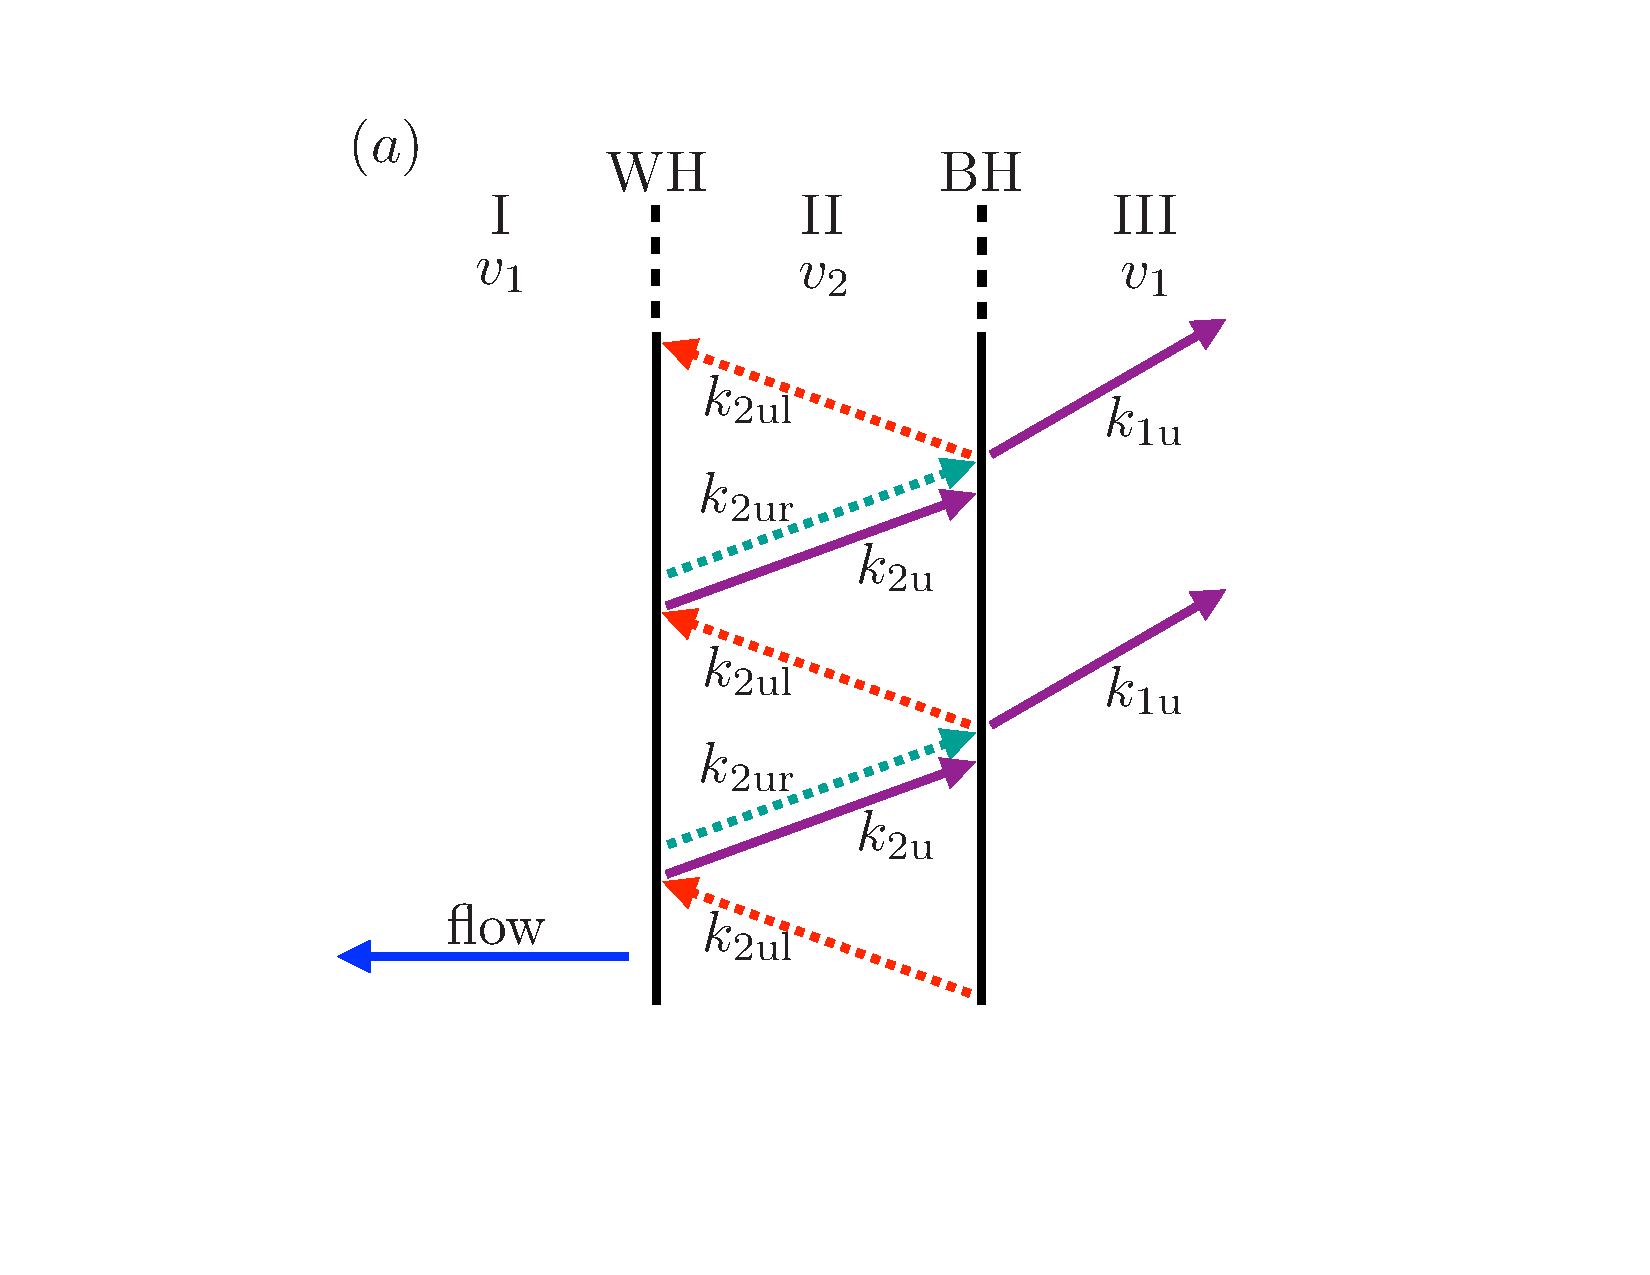
\includegraphics[scale=0.4]{Fig24}
	\caption{Diagrama para la evoluci\'{o}n del modo $k_{2\text{ul}}$ atrapado en la cavidad. Las l\'{i}neas punteadas indican modos con norma negativa y las l\'{i}neas continuas indican modos de norma positiva. Observe que en este an\'{a}lisis no se tienen en cuenta los modos copropagantes indentificados con la etiqueta (v) en la figura \ref{fig:2.1}(a) \citep{2018Bermudez}.}\label{fig:2.2}
\end{figure}

Este modo se encuentra en la rama contrapropagante y se mueve en direcci\'{o}n opuesta al fluido en el marco com\'{o}vil, es decir del $\text{BH}\rightarrow \text{WH}$. Al llegar al $\text{WH}$, este se dispersa creando los modos $k_{2\text{ur}}$ con norma negativa y $k_{2\text{u}}$ con norma positiva, ambos movi\'{e}ndose a la derecha ($d\omega/dk>1$) en direcci\'{o}n al $\text{BH}$. Cuando los modos llegan al horizonte, nuevamente son dispersados cr\'{e}andose el modo $k_{1\text{u}}$ con norma positiva, el cual logra escapar de la cavidad, adem\'{a}s se crea de nuevo el modo $k_{2\text{ul}}$, tal que se conserve la norma. El proceso se repite nuevamente generando as\'{i} un ciclo.\\

Los modos mencionados son creados como consecuencia de la conservaci\'{o}n de la frecuencia en el marco de laboratorio. Adem\'{a}s, por conservaci\'{o}n de la norma la amplitud de los modos aumenta en cada ciclo al mezclarse modos de frecuencia positiva y negativa. La amplificaci\'{o}n puede ser vista entonces como un mecanismo equivalente al funcionamiento de un dispositivo l\'{a}ser, donde la energ\'{i}a con la que se produce la amplificaci\'{o}n proviene de los horizontes producto del cambio de velocidad del fluido en movimiento donde se generan las perturbaciones. El anterior comportamiento del modo $k_{2\text{ul}}$ puede ver resumido en la figura \ref{fig:2.2}.







